\section[Effects on downstream analysis]{Effects of additional somatic variants on downstream analysis}
\label{variantcalling-sec:downstream}

The ability to find additional shared variants significantly impacts our understanding of cancer evolution and the timing of initiation and metastatic seeding. Recent work has shown that, similarly to the well-known genetic heterogeneity, there is heterogeneity regarding the timing of metastatic seeding. While traditionally, it was thought that tumours only metastasise after reaching a certain size to escape the restrictions of the niche, like reduced nutrition, recent publications have shown that there is often very early metastatic seeding \cite{Hu2019}. 
For all methods analysing this heterogeneity, evolutionary timing and history rely entirely on the somatic variants found in the data. Therefore, if we improve the input provided by these analysis methods, we can expect a more precise and possibly more granular result.

The following section will quantify the effect of additionally found variants on phylogenetic reconstruction and clonal decomposition, which use somatic variants as input.

\subsection[Phylogenetic reconstruction]{Phylogenetic reconstruction}
\label{variantcalling-sec:phylo}
As this work is not about the advantages and shortcomings of different phylogenetic reconstruction tools, we have not performed a comprehensive comparison of tools but rather focused on the results of using additional variants discovered using our novel joint somatic variant calling workflow. For this reason, we chose to use neighbour joining (NJ) \cite{Saitou1987} because it is fast and readily available in most phylogenetic reconstruction tool kits, and if the input distance is correct, the output will be correct. Furthermore, even if the distance is not 100\% correct if the distance is ``nearly additive`` and the input distances are not far off from the real distances, the tree topology will still be reconstructed correctly \cite{Mihaescu2007}. Lastly, in contrast to many other methods like UPGMA and WPGMA \cite{Sokal1958}, NJ does not assume an equal mutation rate of each sample because we know that the molecular clock hypothesis \cite{Zuckerkandl1962} is not valid for different lineages of cancers \cite{Shibata2010}.

The only thing that NJ requires as an input is a distance matrix of all samples, so the next step was the selection of the proper distance metric. While there are many distance measures for DNA sequences, which allow accounting for different probabilities of transitions and transversions as well as uneven base composition, models like F81 \cite{Felsenstein1981} or HKY85 \cite{Hasegawa1985} are only really designed for germline mutations and are not \change{easily}{readily} applicable for subclonal somatic mutations. For this reason, we decided \add{first} to \remove{first} transform the variants present in all samples into a binary occurrence vector and then calculate the Hamming distance \cite{Hamming1950} between all samples. This \add{transformation} generates a maximum parsimony approach, and the branch length of the trees will be directly translatable to the \change{amount}{number} of variants which are different between samples. 

\autoref{fig:ca9phylo} shows both the reconstructed phylogenies of the autopsy samples of the previously described late-stage melanoma patient ``CA-F`` from the manuscript (\autoref{ch:appendixManuscript}, \autoref{A:tab:S1}), using the variants found with the default tumour-normal method on the left and our improved joint method on the right. The \remove{exact} same reconstruction methodology was otherwise used.

\begin{figure}[ht]
\centering
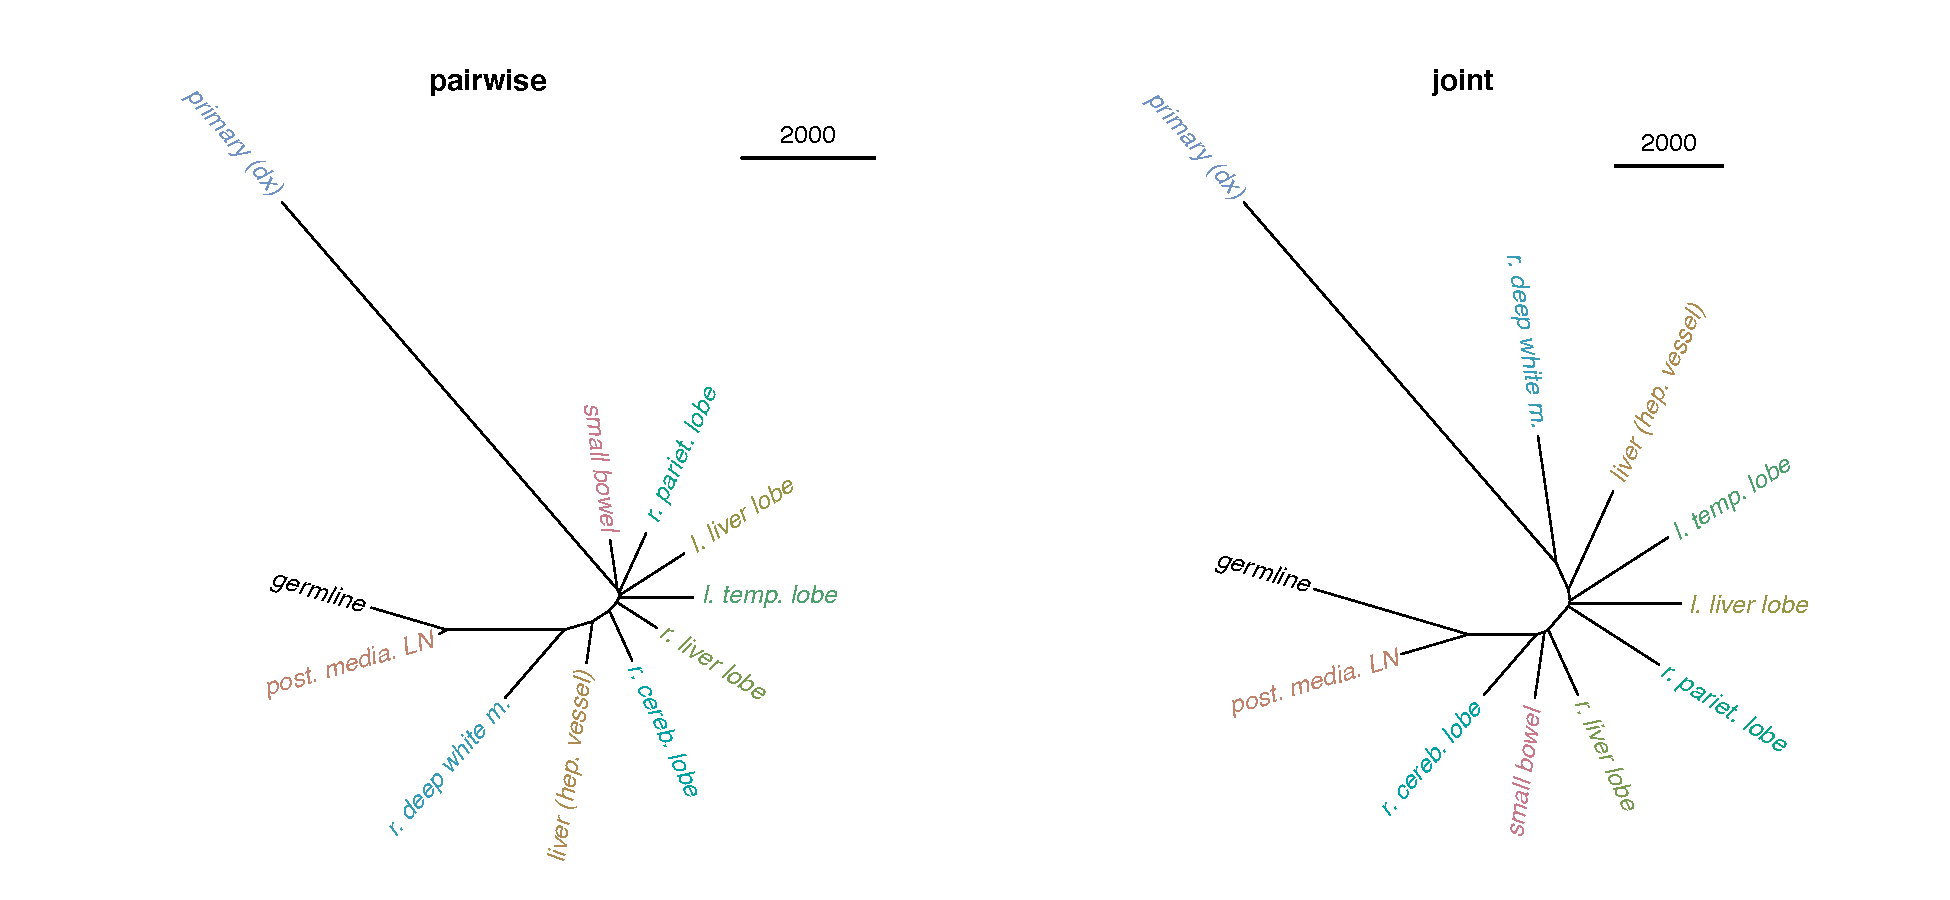
\includegraphics[width=.99\linewidth]{Figures/jointVariantCalling/phyloCA9.pdf}
\caption[Reconstructed phylogenies of joint samples]{Reconstructed phylogenies of a patient with multiple spatially distinct samples; Neighbour joining on Hamming distance on variant occurrence vector. Tip labels describe the location of the sample in the patient. Trees are shown as unrooted with germline as fixated origin point; black line ruler shows the length of an edge with 2000 mutations; LN = lymph node}\label{fig:ca9phylo}
\end{figure}


There are several \change{obvious}{noticeable} differences, first in the longer edge connecting the germline to all other samples, which we consider as the state of no somatic variants. This shows that there are many more shared mutations in all samples than what would have been anticipated with the default method, which corresponds to an overestimation of the heterogeneity of the samples. As the accumulation of somatic variants is still used as a proxy for timing and cell divisions, when assuming a high mutation rate for lung cancer ($5.3 \cdot 10^{-8}$ from \citeauthor*{Werner2020} \cite{Werner2020}) this difference of $\approx 36000$ variants is equivalent to $\approx 2000$ cell divisions. While the cell doubling rate of cancers is highly dependent on the type \cite{Arai1994}, this change makes a substantial difference when assessing the timing of the tumour initiation and further evolution. 

Secondly, there have been topological changes, which generate a longer bifurcating edge between the olive-coloured ``right liver lobe`` and the ``right parietal lobe`` lesions showing a bottleneck in cancer evolution, which corresponded with the clinical history, where the patient lived with stable disease for almost ten years, before rapid disease progression just prior to death. \add{Finally,} the extreme distance of the primary/diagnostic sample from the rest of the samples could be in part due to a difference in sequencing quality, as this was an FFPE tumour biopsy. However, as this feature is preserved between \remove{both} the joint and the pairwise analysis, it does not appear to be an effect of our new method.

\begin{figure}[ht]
\centering
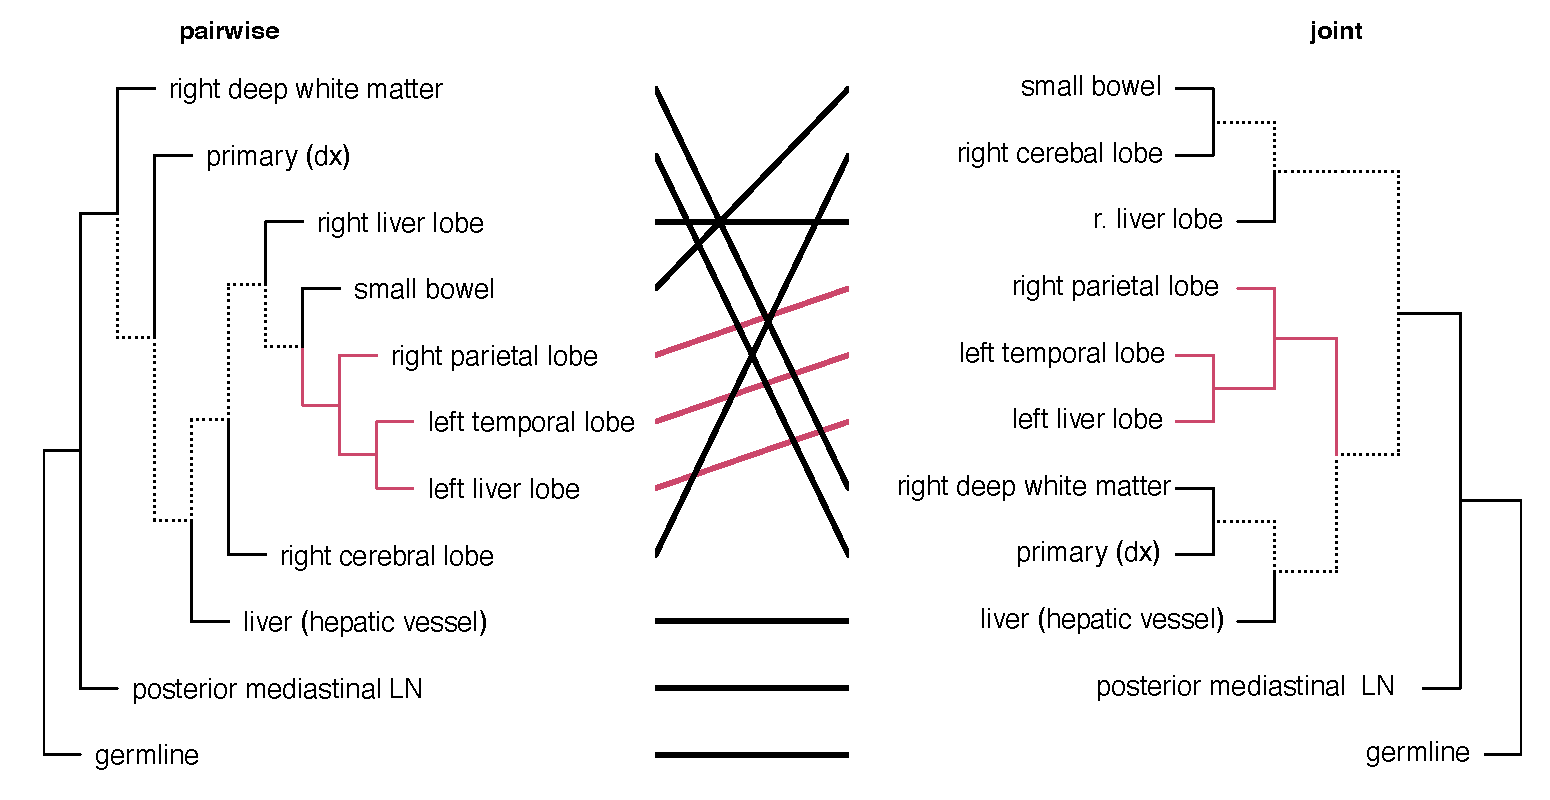
\includegraphics[width=.99\linewidth]{Figures/jointVariantCalling/tanglePhyloCA9.pdf}
\caption[Tanglegram of the reconstructed phylogenies]{Side by side view of the reconstructed trees from \autoref{fig:ca9phylo}; internal edges, which are distinct between trees are shown as dotted lines; common subtree is shown in red  Tree labels have been sorted to minimise distance between labels; LN = lymph node ; Visualisation generated with dendextend \cite{Galili2015}}\label{fig:tanglePhyloCA9}
\end{figure}

\autoref{fig:tanglePhyloCA9} shows a topology-focused view of the two phylogenetic trees, \remove{which} highlight\change{s}{ing} the differences between the two reconstructions \cite{Vienne2018}. The common subtrees are coloured the same on both sides, and connecting lines show identical labels. This format shows that while the trees look quite similar at first glance, they show vastly different topologies.


One example of this is the ``small bowel`` tumour sample which was originally connected to the \remove{red} common \add{red} subtree but is now much closer to the ``right cerebral lobe`` lesion, forming a parallel clade with the ``right liver lobe`` lesion. In general, whereas the pairwise tree shows a very linear topology with minimal branching and no disjunct subclades, these features are \remove{clearly} present in the joint reconstruction.  (\autoref{fig:tanglePhyloCA9}).


\section[Longitudinal analysis]{Longitudinal analysis}
\label{variantcalling-sec:longitudinal}

In addition to the analysis of spatial heterogeneity through multi-regional tu\-mour sam\-pling, we were also interested in \change{the use of}{using} our novel joint variant calling workflow \change{for the analysis of}{to analyse} temporal heterogeneity through longitudinal samples collected from the same patient over time. Examples of longitudinal analysis could include the joint analysis of diagnostic and relapse tumour tissue samples or even the repeated serial testing of ctDNA. In the following section, we present work using the published workflows on a longitudinal dataset, \change{which highlights the}{highlighting the new methods'} flexibility and widespread usability \remove{of the new methods}. Similar to the spatially related samples, the joint analysis can improve the performance, which then in turn enables improved detection of lower allele frequency variants, particularly in the setting of low tumour burden, as is commonly seen with ctDNA analysis.

In addition to their autopsy, which resected nine distinct tumour sites (\autoref{fig:CA-Fschematic}), Patient ``CA-F`` also had three longitudinal blood samples taken, from which ctDNA was extracted, and WES performed. These blood samples were taken as non-invasive surveillance seven, five and two months before the \change{death of the patient}{patient's death} (\autoref{fig:CA-Ftimeline}).

\begin{figure}[ht]
\centering
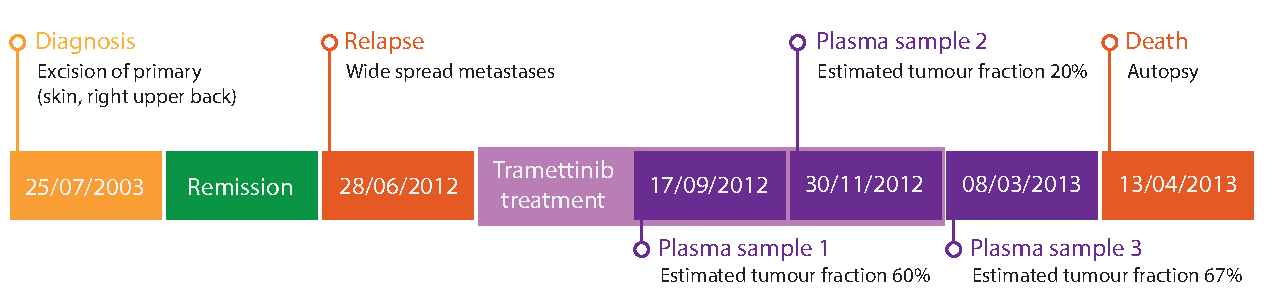
\includegraphics[width=.99\linewidth]{Figures/jointVariantCalling/CA-F_timeline.pdf}
\caption[Timeline from diagnosis till death for patient CA-F]{Timeline from diagnosis till death for patient CA-F: 1.9mm melanoma removed after diagnosis \formatdate{25}{07}{2003} but with negative sentinel lymph node biopsy; \formatdate{28}{06}{2012}: PET scan and subsequent liver biopsy confirm relapse with wide spread metastases; trametinib treatment from Oct. 2012 till Jan. 2013 with minor response; blood plasma samples during treatment (1 and 2) as well as after progression (3); death and rapid autopsy of nine metastatic sites (\formatdate{13}{04}{2013}, \protect\autoref{fig:CA-Fschematic}); Tumour fraction in plasma samples was estimated via digital droplet PCR quantification of the original driver mutation (BRAF:K601E)}\label{fig:CA-Ftimeline}
\end{figure}

\begin{figure}[ht]
\centering
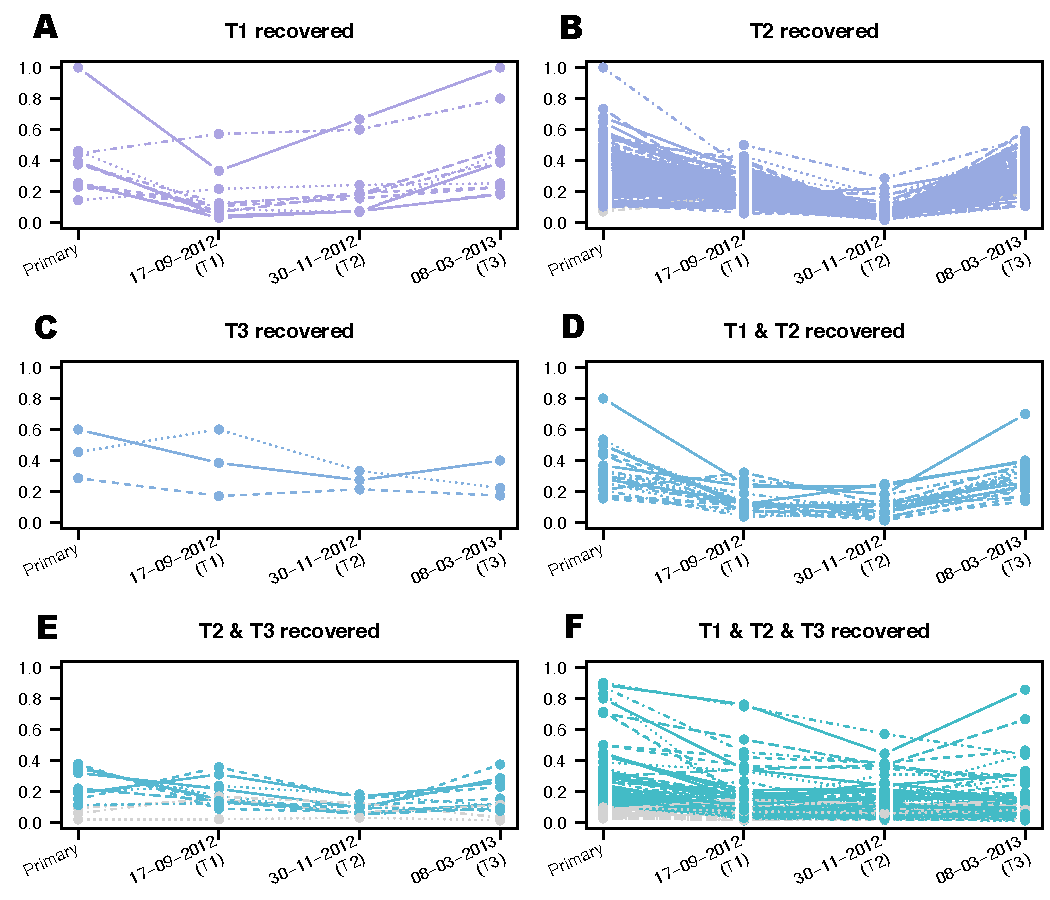
\includegraphics[width=.99\linewidth]{Figures/jointVariantCalling/longitudinalCA9ctDNAVafs.pdf}
\caption[Improved somatic variant calling in longitudinal data]{Improved somatic variant calling in longitudinal data: Variant allele frequency (VAF) of variants found additionally through joint variant calling which were found as high confidence variants in the primary sample; Variants with less than 0.1 VAF in the primary are coloured grey; ``T1 recovered`` shows variants, which were high confidence in all ctDNA samples but T1 and were only found through joint calling there; Axis label show the date of blood collection }\label{fig:longitudinalVAFsctDNA}
\end{figure}

To show that even in longitudinal data, the joint analysis can boost the signal, we jointly variant called variants in the diagnostic biopsy sample with the three ctDNA samples and compared them with the results from the pairwise analysis. On average, we found 2905 additional variants in each \remove{of the} ctDNA sample\remove{s}, which is more than doubles the average number of variants found with the pairwise analysis (2414). Out of those, we found 534 ($\approx 20\%$) variants in the ctDNA samples, which were found as a high confidence variant in the diagnostic sample, indicating that these findings were high-quality calls. 

As in the spatial\remove{ly} analysis, in longitudinal data, lower tumour purity samples benefit more from the joint analysis. We see that time point 2 (T2) had the highest number of recovered variants (377) which were found as high confidence variants in both other time points (\autoref{fig:longitudinalVAFsctDNA} A vs. B vs. C), and T2 also has the lowest ctDNA fraction recorded (T1: 60\%; T2: 20\%; T3: 60\%). A total of 106 variants were not found in the ctDNA samples with the pairwise analysis, even though they were high-confidence variants in the primary sample (\autoref{fig:longitudinalVAFsctDNA}F). These variants usually showed a lower depth of coverage (\change{dp}{DP}) in the ctDNA samples, which is likely the explanation as to why they were below the limit of detection of the pairwise analysis. 

\begin{figure}[ht]
\centering
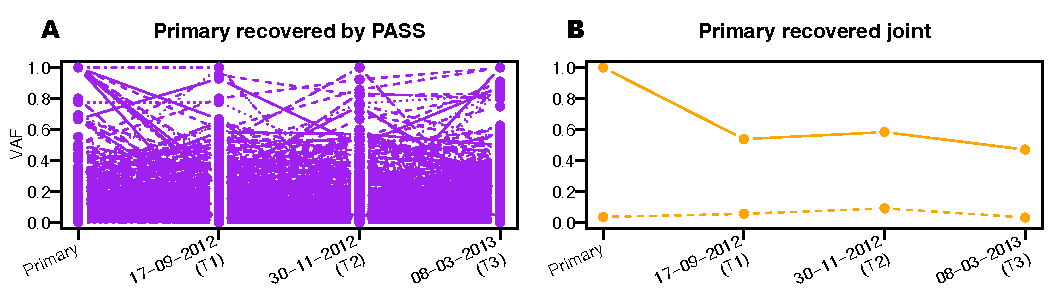
\includegraphics[width=.99\linewidth]{Figures/jointVariantCalling/longitudinalCA9primaryVafs.pdf}
\caption[Longitudinal data informs diagnostic variant calling]{Longitudinal data informs diagnostic variant calling: VAFs of variants additionally found through joint calling in the primary samples; A) ``Primary recovered by PASS`` shows variants which were high confidence in at least one ctDNA sample but not found in the primary; B) ``Primary recovered joint`` shows variant which were low confidence in all samples in the pairwise analysis individually but were called as high confidence in the joint analysis; Axis label show the date of blood collection}\label{fig:longitudinalVAFsprimary}
\end{figure}

Finally, we can also find 398 additional variants in the primary sample. All but two of these variants were discarded in the pairwise analysis due to low evidence in the tissue sample, but could be found with a high confidence in the longitudinal data. The last two variants \remove{were} could be found in the joint analysis, as all 4 samples showed evidence for these variants just below the limit of detection. \add{This is especially surprising as the variant allele frequency in the normal sample is 100\%, however only 4 reads cover this variant in the tissue sample and an average of 5.8 in the ctDNA samples} (\autoref{fig:longitudinalVAFsprimary}). \note{adjusted figure labels}

These additional findings shows that both spatially and longitudinal related samples should be analysed jointly, as it substantially increases the \change{amount}{number} of true variants found, which can \change{have a large impact on}{greatly impact} the downstream analysis of the samples.



\subsection[Clonal deconvolution]{Clonal deconvolution}
\label{variantcalling-sec:clonal}

One of the most important pieces of information \remove{that can be} derived from multiple related samples from the same patient is the clonal deconvolution, where subclonal reoccurring patterns of mutations (clones) are resolved \remove{both} spatial\remove{ly} and longitudinal\remove{ly}. These reoccurring clones can be linked to either parallel evolution through positive selection pressure, like a targeted drug, or due to the process of developing metastases where a part of the cancer disseminates and grows at a different site.
In contrast to the lack of options for joint somatic variant calling, \change{there is a plethora of}{many} algorithms and methods \add{are} available for clonal deconvolution. Since 2015 PhyloWGS \cite{Deshwar2015}, Canopy \cite{Jiang2016}, CLOE \cite{Marass2016}, CloneFinder \cite{Miura2018}, MACHINA \cite{ElKebir2018} and MOBSTER \cite{Caravagna2020} \change{were}{have been} published, to name a few. Underlying all of these models is the ability to cluster variants with similar variant allele frequencies together to reduce the combinatorial space and enhance the confidence in the signal \cite{Tarabichi2021}. \add{However,} due to the high number of tools, it is very challenging to select the right tool, especially since all of them have advantages and disadvantages \cite{Miura2020}. In this work, we decided to use PhylogicNDT \cite{Leshchiner2018} as it has been shown to work well on clinical samples \cite{Gerstung2020} and does not have the restriction for the input to be from copy number neutral areas, which many of the other tools have.


Both the variants found with the default pairwise as well as with the new joint workflows were annotated with their local allele-specific copy number to form a MAF-like file format \change{which}{that} \remove{is required by} PhylogicNDT \add{requires}. While PhylogicNDT allows the user to supply the cancer cell fraction for every variant, the program can also estimate them from the supplied allelic counts and the copy number. Local copy number calls were derived from copy number segment calls made by Sequenza by intersecting the chromosomal location of each variant with the copy number segment containing the variant's location. This \add{annotation} requires multiple steps, and the source code is shown in \autoref{lst-jvcAppendix:parseVcf} (parsing VCF), \autoref{lst-jvcAppendix:cnv} and \autoref{lst-jvcAppendix:convertMAF} (convert to MAF format). Variants \change{which}{that} could not be annotated with copy number information because their genomic location did not overlap with any called copy number segment were discarded for this analysis.

\begin{figure}[ht]
\centering
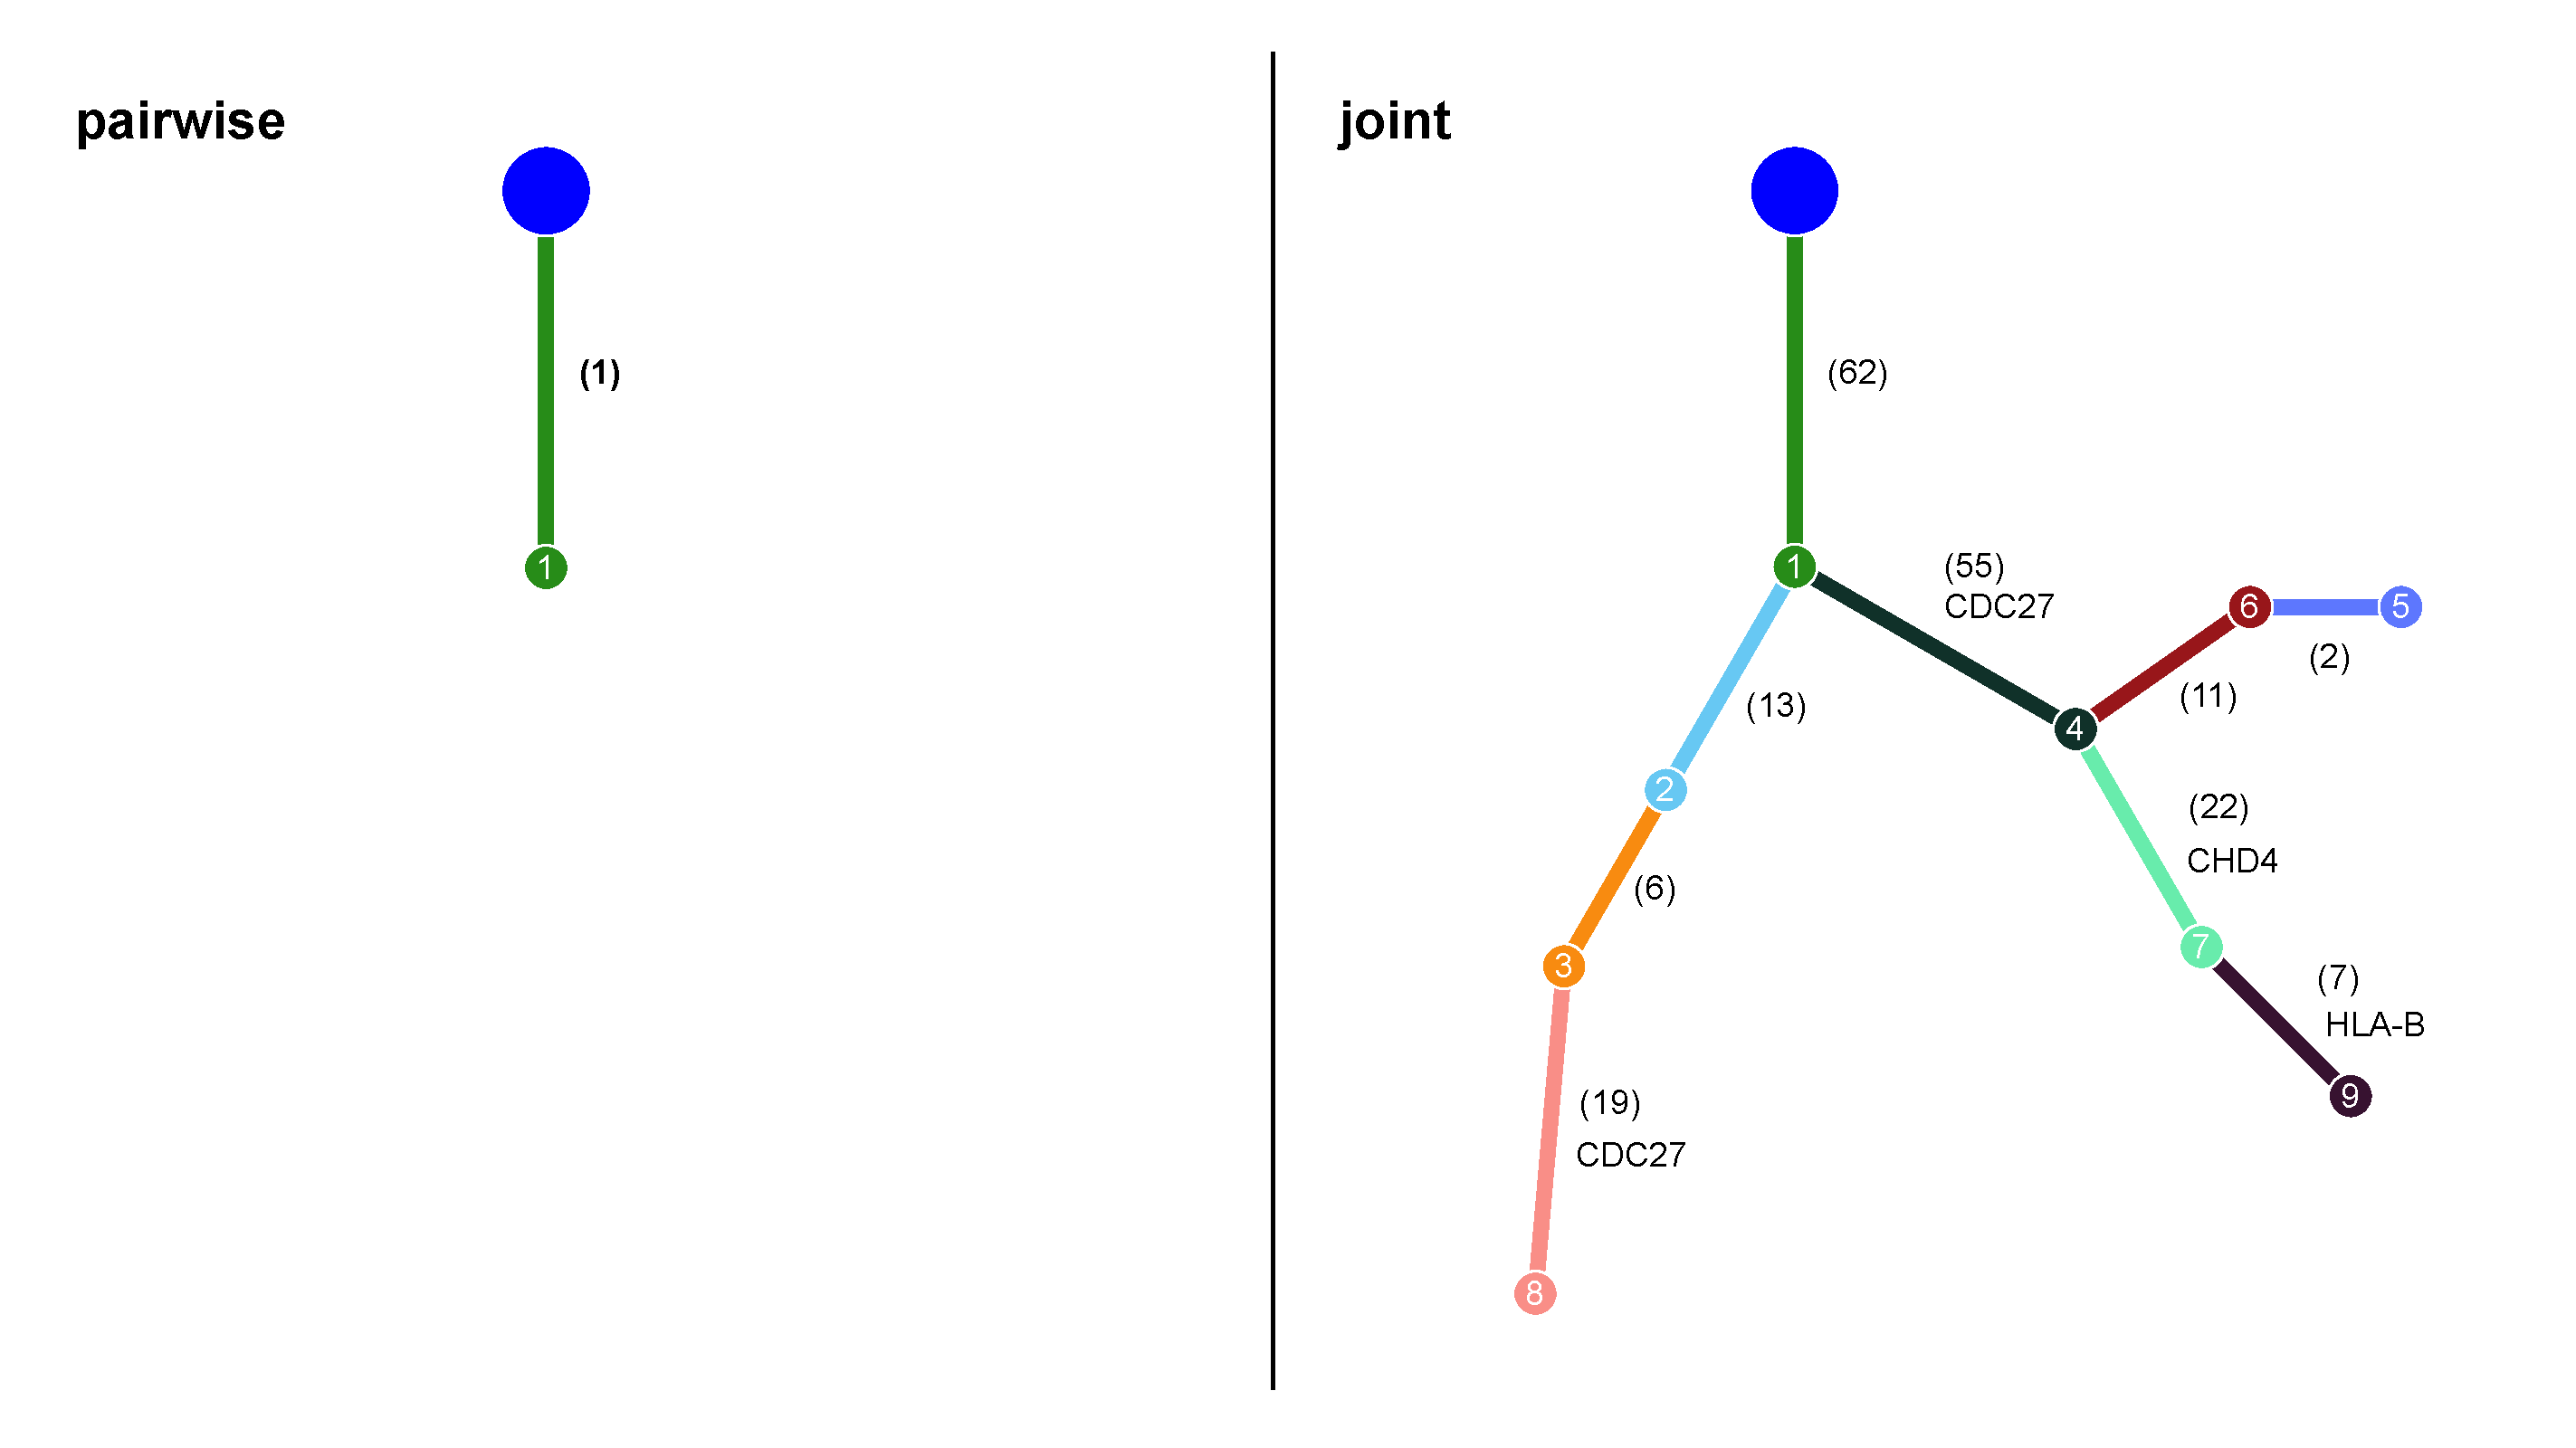
\includegraphics[width=.99\linewidth]{Figures/jointVariantCalling/clonalDeconv.pdf}
\caption[Reconstructed clonal trees for joint and pairwise variant calling]{Reconstructed clonal trees from PhylogicNDT; Blue circle at top depicts the germline/normal state. The coloured edges with the same coloured circle represents a distinct subclone of the parent from which the edge emerges; The number in braces next to the edge is the number of mutations which define this subclone with an added gene symbol added, if there was a cancer driver gene mutation. The left part shows the result when using the default pairwise method of Strelka2 and the right side uses the results from the Strelka2Pass workflow}\label{fig:clonaldeconv}
\end{figure}


\autoref{fig:clonaldeconv} shows the highest parsimony clonal tree reconstructed by PhylogicNDT for the pairwise \change{as well as}{and} the joint variant calling for patient CA-F. As the copy number calling information is the same for both inputs, the only difference is in the called variants. While there was no subclonal structure detected \remove{at all} for the pairwise analysis, \remove{there is} a highly complex branching structure \add{was} detected using the jointly called variants with multiple subclones originating from the ancestral clone. As this is a clinical sample, we cannot be \change{certain}{sure} that the more branched model is the actual truth, but it is biologically more logical that a late-stage cancer has developed several subclones rather than it being a very homogeneous disease at all of the ten sites at autopsy with no evolution over ten years of disease \cite{Gerstung2020}.
It is of particular interest that the \textit{CDC27} gene was mutated at different time points in different clones (clone 8 vs. clone 4), which is a clear indicator of convergent evolution, which would \remove{definitely} be missed without the joint analysis.


\subsection{Longitudinal enriched phylogeny}
\label{variantcalling-sec:fullphylo}
Of course, it is finally also possible to build a phylogeny \change{which}{that} incorporates data from both the spatial tumour tissue and longitudinal ctDNA analysis. However, as the ctDNA can provide a holistic view of all cancer metastases (\autoref{intro-sec:ctDNA}), the interpretation needs to accommodate \remove{for} that. 

\begin{figure}[ht]
\centering
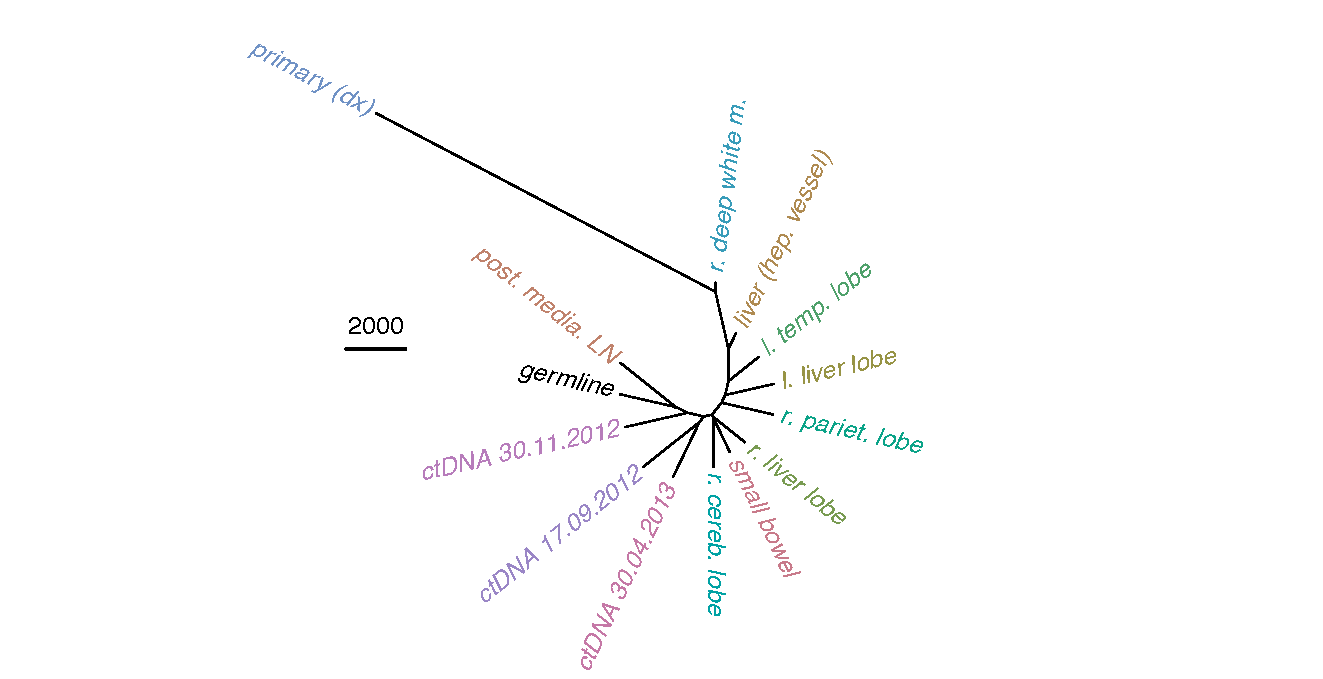
\includegraphics[width=.99\linewidth]{Figures/jointVariantCalling/phyloCA9_withctDNA.pdf}
\caption[Reconstructed phylogeny with longitudinal ctDNA samples]{Reconstructed phylogeny with longitudinal ctDNA samples: Tree from \autoref{fig:ca9phylo} with three additional ctDNA samples from different time points approximately one year prior to death. The ruler shows the equivalent of 2000 mutations; LN = lymph node} \label{fig:phyloCA9ctDNA}
\end{figure}

The addition of the ctDNA samples led to a further bipartition edge, which separates the ``right liver lobe``, ``small bowel``, and ``right cerebral lobe`` lesions from the rest of the tree (\autoref{fig:phyloCA9ctDNA}). This separation was already inferable from the topology of the previous tree in \autoref{fig:tanglePhyloCA9} ``joint``, but is even more pronounced with the inclusion of the ctDNA samples.

This result shows that \change{the addition of}{adding} more samples helps to refine and improve the trajectory and history of cancer samples, and it is vital to do this analysis jointly to generate the optimal result.